\chapter{Fundamentos teóricos}
\label{cap:fundamentos_teoricos}
Este capítulo se enfoca en analizar en profundidad los aspectos técnicos necesarios para llevar a cabo el desarrollo del CanSat.
Se incluye una comparativa entre los distintos microcontroladores y microcomputadores disponibles en el mercado, evaluando su precio, disponibilidad y adecuación a los requisitos técnicos del proyecto.
Además, se analizan los sensores y módulos de comunicación más comunes, así como los principales protocolos utilizados para la comunicación entre el microcontrolador y los sensores, como I2C y UART.
También se estudian distintas opciones para la retransmisión de vídeo en tiempo real desde el CanSat.
Por último, se exploran soluciones para la visualización de los datos a través de una interfaz web en tiempo real.


\section{Comparativa de microcontroladores y microcomputadores}
Uno de los componentes principales de un CanSat o de cualquier sistema embebido en general es su microcontrolador o microcomputador,
es el encargado de comunicarse con los sensores, procesar los datos y transmitirlo a través del módulo de comunicación,
también es el encargado de procesar el video y retransmitirlo en tiempo real(si el hardware lo permite).

Primero conviene aclarar la diferencia entre microcontrolador y microcomputador:
\begin{itemize}
    \item \textbf{Microcontrolador:} Circuito integrado que combina procesador, memoria y periféricos de entrada/salida en un solo chip.
    Está diseñado para realizar tareas específicas con bajo consumo energético y recursos limitados.
    Es común en aplicaciones como lectura de sensores, control de motores o gestión de comunicaciones básicas.
    Ejemplos comunes son Arduino Uno o ESP32
    \item \textbf{Microcomputador:} Sistema completo en una sola placa (Single-Board Computer) que integra procesador, memoria, almacenamiento y puertos de expansión.
    Es capaz de ejecutar sistemas operativos completos (como Linux) y realizar tareas más complejas, como procesamiento de imágenes, servidor web o interfaces gráficas.
    Un ejemplo típico es la Raspberry Pi Zero.
\end{itemize}

Actualmente, en el mercado se pueden encontrar varios de estos microcontroladores o microcomputadores de bajo coste, tamaño y peso reducido y bajo consumo.
En esta sección nos vamos a centrar en el análisis de tres de las opciones más populares:
\begin{itemize}

    \item \textbf{\cite{raspberrypi_zero2}:}
    La Raspberry Pi Zero 2 es un Single Board Computer de bajo costo lanzado en Reino Unido por la~\cite{raspberrypi_foundation},
    de toda la familia Raspberry Pi se ha elegido el modelo Zero 2 por ser el de tamaño más reducido pero con una potencia adecuada para el desarrollo de un proyecto como el CanSat.
    Las características más relevantes para este proyecto son:
    \begin{itemize}
        \item CPU Arm Cortex-A53 de cuatro núcleos y 64 bits a 1 GHz.
        \item SDRAM de 512 MB.
        \item LAN inalámbrica de 2,4 GHz 802.11 b/g/n.
        \item Bluetooth 4.2, Bluetooth Low Energy (BLE), antena integrada.
        \item Ranura para tarjeta microSD.
        \item Conector de cámara CSI-2.
        \item Cabecera GPIO de 40 pines para conexión de periféricos.
        \item 1 × SPI
        \item 2 × interfaces I²C
        \item 1 × UART
        \item Consumo típico de energía: entre 0.7\,W y 1.5\,W dependiendo de la carga de trabajo.
        \item Precio aproximado: 15–20€.
    \end{itemize}
    \begin{figure}[h]
        \centering
        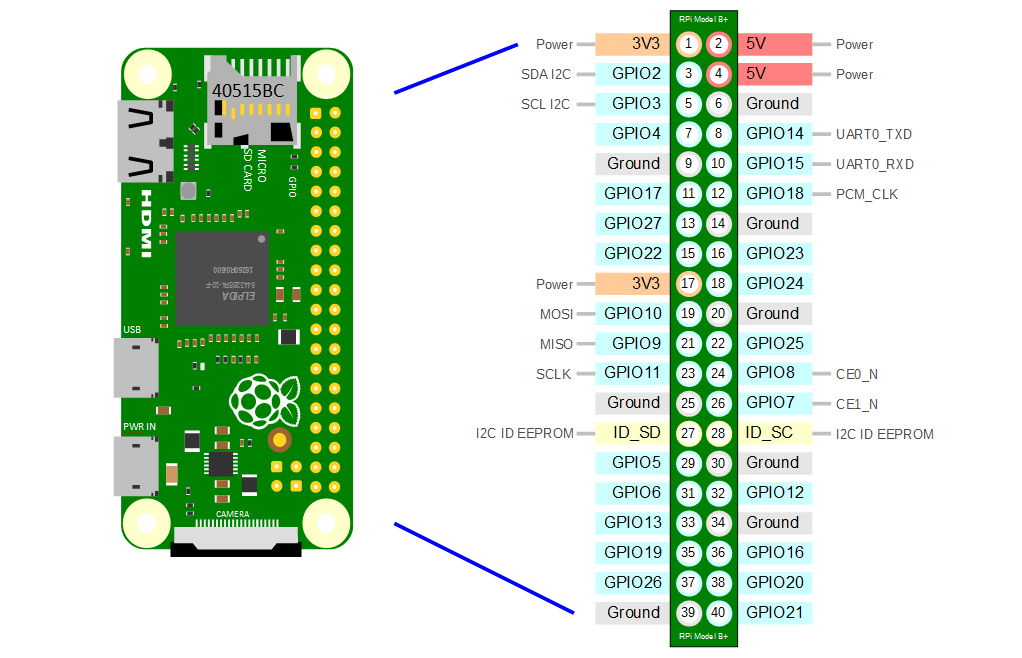
\includegraphics[width=0.8\textwidth]{Imagenes/Bitmap/pizero2gpio}
        \caption{Distribución de pines GPIO en Raspberry Pi Zero 2}
        \label{fig:pizer2_gpio}
    \end{figure}
    Como se puede ver en las características la Raspberry Pi Zero 2 cumple con los requisitos necesarios para este proyecto,
    cuenta con un procesador y memoria adecuados, soporte para cámara (útil para la retransmisión de video en tiempo real), conectividad inalámbrica mediante WiFi
    y compatibilidad con los protocolos I\textsuperscript{2}C y UART mediante los pines GPIO necesarios para la conexión directa de sensores.

    \item \textbf{\cite{esp32}:}
    Es un microcontrolador de bajo coste desarrollado por Espressif Systems que combina bajo coste con buena capacidad de procesamiento y conectividad inalámbrica integrada,
    lo que lo convierte en una de las opciones más populares para proyectos embebidos, incluyendo CanSat.

    A diferencia de un microcomputador como la Raspberry Pi, el ESP32 no ejecuta un sistema operativo generalista,
    pero su bajo consumo energético y la integración de múltiples periféricos lo hacen convierten en muy buena opción cuando se busca eficiencia y simplicidad del sistema.

    Las características más relevantes para este proyecto son:
    \begin{itemize}
        \item CPU dual-core Tensilica Xtensa LX6 a 240\,MHz.
        \item 520\,KB de SRAM interna.
        \item Memoria flash externa: normalmente 4\,MB (dependiendo del modelo).
        \item Conectividad Wi-Fi 802.11 b/g/n.
        \item Bluetooth 4.2 y BLE.
        \item 4 × SPI
        \item 2 × interfaces I²C
        \item 3 × UART
        \item Hasta 34 pines GPIO (según versión del módulo).
        \item Consumo típico: entre 0.2\,W y 0.6\,W, dependiendo del modo de operación.
        \item Precio aproximado: 4–8€~\cite{esp32}.
    \end{itemize}
    \begin{figure}[h]
        \centering
        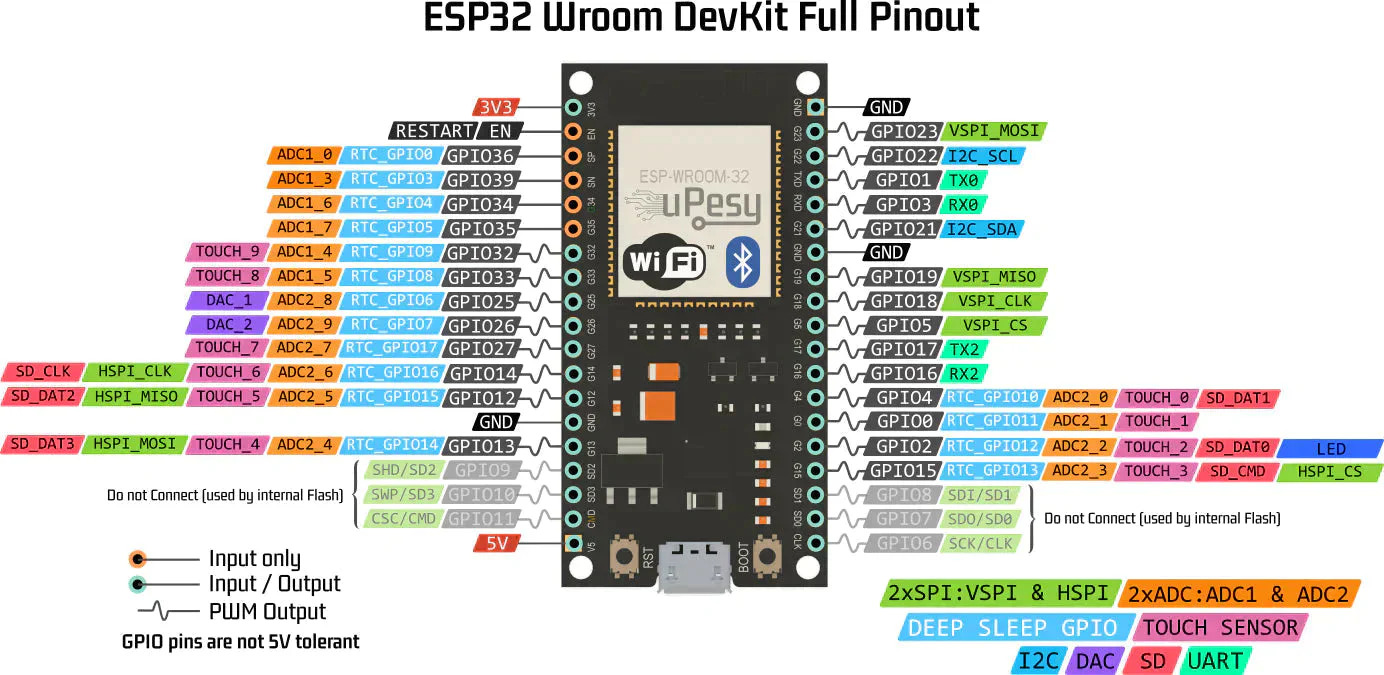
\includegraphics[width=0.8\textwidth]{Imagenes/Bitmap/esp32gpio}
        \caption{Distribución de pines GPIO en ESP32}
        \label{fig:esp32gpio}
    \end{figure}

    Gracias a su bajo consumo, potencia y multiples conexiones, el ESP32 permite integrar sensores fácilmente a través de interfaces estándar y puede encargarse tanto de la adquisición como de la transmisión de datos por radio o Wi-Fi.
    Además, su bajo consumo lo hace especialmente adecuado para sistemas alimentados por batería en entornos con restricciones energéticas.
    También existen variantes como el ESP32-CAM que integran una cámara de tipo OV2640, lo que permite capturar imágenes y transmitir video mediante Wi-Fi
    aunque con un rendimiento y resolución inferior a la de Raspberry Pi.

    \item \textbf{\cite{arduino_nano}:}
    Es un microcontrolador compacto de bajo coste basado en el chip ATmega328P, es el más utilizado en entornos educativos gracias a su simplicidad,
    por lo que cuenta con una amplia comunidad detrás y desarrollo de librerias.
    A diferencia de la Raspberry Pi Zero 2 o el ESP32, el Arduino Nano no cuenta con conectividad inalámbrica ni capacidad de procesamiento avanzada,
    pero es suficiente para gestionar sensores básicos y transmitir datos mediante un módulo externo de radio.

    Las características más relevantes para este proyecto son:
    \begin{itemize}
        \item Microcontrolador ATmega328P.
        \item Frecuencia de reloj: 16\,MHz.
        \item Memoria flash: 32\,KB (2\,KB utilizados por el bootloader).
        \item SRAM: 2\,KB.
        \item EEPROM: 1\,KB.
        \item 22 pines GPIO (14 digitales, 8 analógicos).
        \item 1 × interfaz I²C.
        \item 1 × UART.
        \item 1 × SPI.
        \item Consumo típico: entre 0.05\,W y 0.2\,W.
        \item Precio aproximado: 27€ en la web oficial.
    \end{itemize}

    \begin{figure}[h]
        \centering
        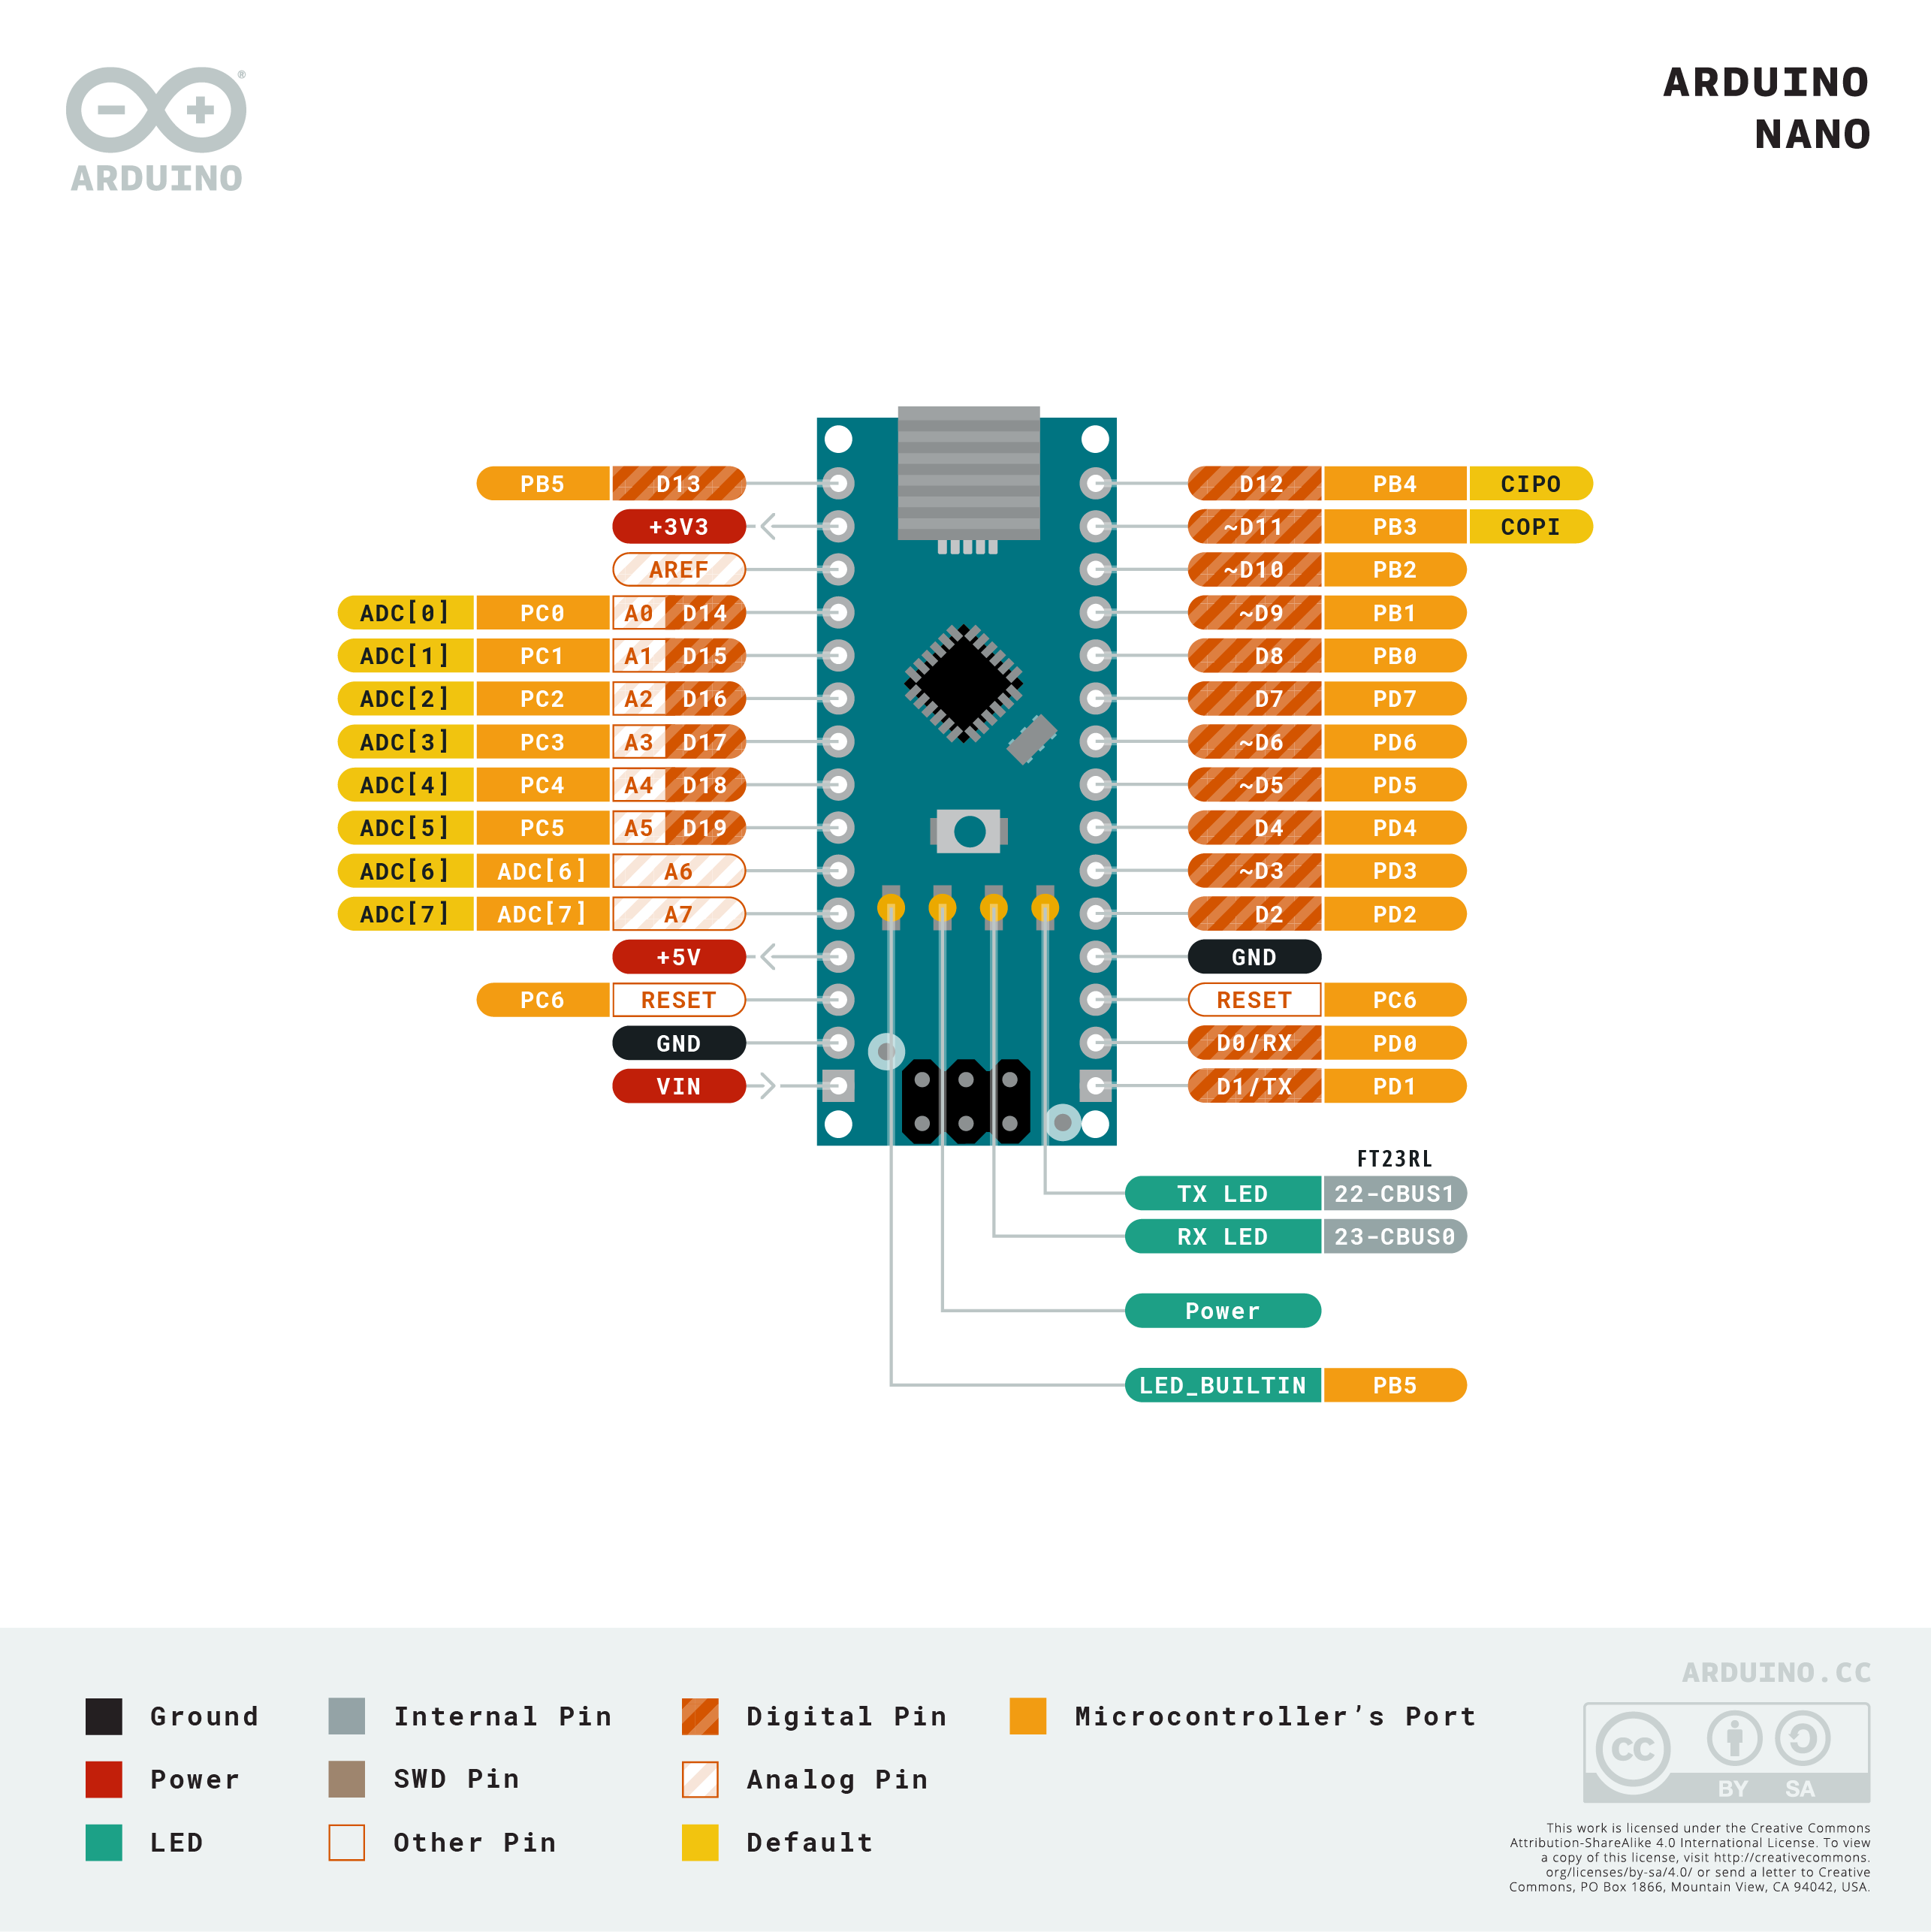
\includegraphics[width=0.7\textwidth]{Imagenes/Bitmap/arduinoNanogpio}
        \caption{Distribución de pines en Arduino Nano}
        \label{fig:arduino_nano_gpio}
    \end{figure}

    Aunque no tiene las capacidades de procesamiento de una Raspberry Pi ni la conectividad integrada del ESP32, el Arduino Nano puede ser una solución válida para CanSat muy simples,
    en los que se priorice el consumo mínimo y no se necesiten funcionalidades avanzadas como WiFi o procesamiento de vídeo, sin embargo, al no tener soporte para cámaras,
    no cumple con los requisitos técnicos necesarios para este proyecto.

\end{itemize}

\begin{table}[h]
    \centering
    \footnotesize
    \begin{tabular}{|l|l|l|l|}
        \hline
        \textbf{Característica} & \textbf{Raspberry Pi Zero 2} & \textbf{ESP32}           & \textbf{Arduino Nano}   \\
        \hline
        Procesador              & ARM Cortex-A53 (4×, 1 GHz)   & Xtensa LX6 (2×, 240 MHz) & ATmega328P (1×, 16 MHz) \\
        \hline
        Memoria                 & 512 MB SDRAM                 & 520 KB SRAM + 4 MB Flash & 2 KB SRAM + 32 KB Flash \\
        \hline
        Wi-Fi                   & Sí                           & Sí                       & No                      \\
        \hline
        Bluetooth               & 4.2 + BLE                    & 4.2 + BLE                & No                      \\
        \hline
        SPI                     & 1                            & 4                        & 1                       \\
        \hline
        I²C                     & 2                            & 2                        & 1                       \\
        \hline
        UART                    & 1                            & 3                        & 1                       \\
        \hline
        Compatibilidad cámara   & CSI (cámara oficial)         & OV2640 (ESP32-CAM)       & No                      \\
        \hline
        Consumo típico          & 0.7--1.5 W                   & 0.2--0.6 W               & 0.05--0.2 W             \\
        \hline
        Precio estimado         & 15--20 €                     & 4--8 €                   & 25--30 €                \\
        \hline
    \end{tabular}
    \caption{Comparativa de microcontroladores y microcomputadores}
    \label{tab:comparativa-mcus}
\end{table}


\section{Interfaces de comunicación serie}
Una vez analizados sobre los distintos microcontroladores y microprocesadores que existen en el mercado para este tipo de proyectos,
es importante entender los distintos tipos de interfaces de comunicación que utilizan para interactuar con sensores y otros módulos externos y como funcionan.
En esta sección se presentan tres de los más relevantes: SPI, I²C y UART

\begin{itemize}
    \item \textbf{SPI:} La interfaz SPI (Serial Peripheral Interface)~\cite{dhaker_spi} es una interfaz síncrona y full dúplex basada en una arquitectura maestro-esclavo,
    los dos dispositivos, maestro y esclavo pueden transmitir datos simultáneamente sincronizados con una señal de reloj.
    La interfaz SPI utiliza cuatro señales:
    \begin{itemize}
        \item Señal de reloj (CLK)
        \item Selección de chip (CS)
        \item Salida del maestro hacia el esclavo (MOSI)
        \item Salida del esclavo hacia el maestro (MISO)
    \end{itemize}
    \begin{figure}[h]
        \centering
        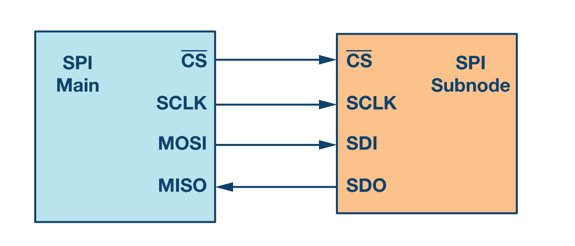
\includegraphics[width=0.8\textwidth]{Imagenes/Bitmap/spi}
        \caption{Configuración SPI con un maestro y un esclavo}
        \label{fig:spi}
    \end{figure}
    El maestro genera la señal de reloj y controla el intercambio de datos.
    El pin CS selecciona el estado activo y los pines MISO y MOSI transportan datos en ambas direcciones.
    Para iniciar la comunicación, el maestro activa el pin CS y empieza a emitir la señal de reloj, al ser una interfaz full dúplex,
    maestro y esclavo pueden enviar y recibir datos simultáneamente.
    Esta interfaz tiene un solo maestro y puede tener uno o múltiples esclavos.
    En configuraciones con múltiples esclavos se pueden conectar de dos modos:
    \begin{itemize}
        \item \textbf{Modo regular:} Cada nodo tiene su propia línea de CS
        \item \textbf{Modo cadena (daisy-chain):} Todos los nodos comparten el mismo reloj y CS y los datos se propagan de un esclavo al siguiente.
        De esta manera se reduce el número de GPIO necesarios en el maestro, aunque aumenta el número de ciclos de reloj requeridos para llegar a cada esclavo.
    \end{itemize}
    La velocidad de transferencia puede variar dependiendo del hardware utilizado, lo habitual es entre 1 y 10Mbps, aunque algunos dispositivos permiten velocidades superiores.

    \item \textbf{I²C:} La interfaz I²C (Inter-Integrated Circuit)~\cite{i2c_specification} es un bus de comunicación síncrono y half dúplex basado en una arquitectura maestro-esclavo, que utiliza solo dos líneas para comunicarse con múltiples dispositivos,
    originalmente fue desarrollada por Philips Semiconductors en 1982.
    Esta interfaz utiliza solo dos señales:
    \begin{itemize}
        \item Línea de datos (SDA)
        \item Línea de reloj (SCL)
    \end{itemize}
    \begin{figure}[h]
        \centering
        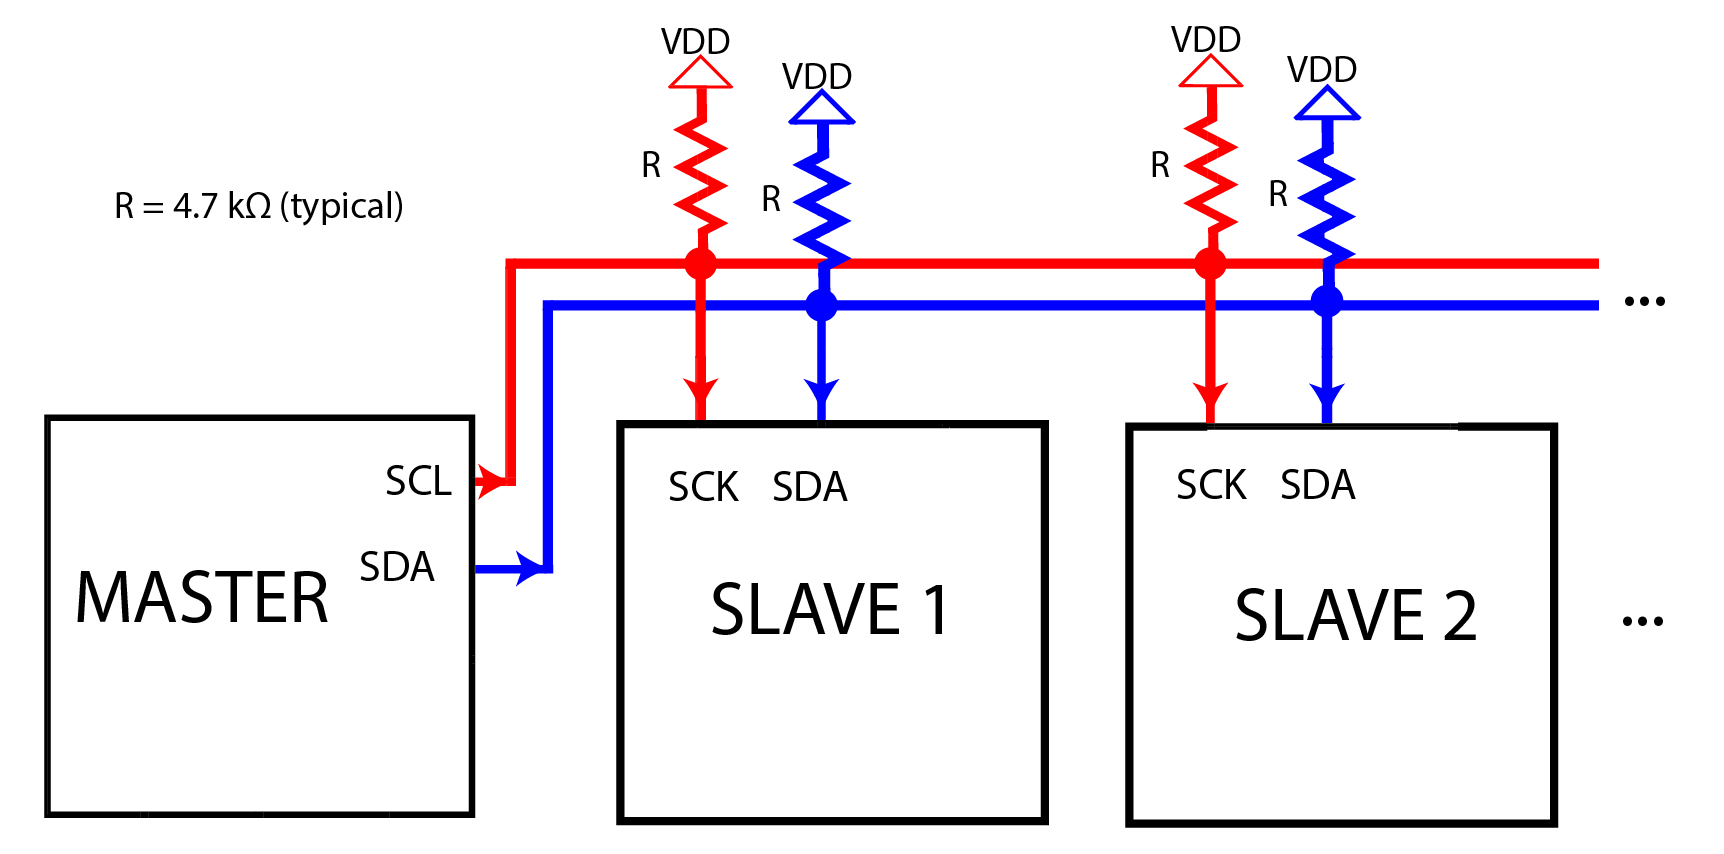
\includegraphics[width=0.8\textwidth]{Imagenes/Bitmap/i2c}
        \caption{Configuración I²C con un maestro y varios esclavos}
        \label{fig:i2c}
    \end{figure}
    Ambas líneas son bidireccionales aunque al ser half dúplex la comunicación se realiza en un sentido a la vez.
    Un dispositivo actúa como maestro, iniciando la comunicación y generando la señal de reloj, mientras que uno o más esclavos responden.
    Cada dispositivo conectado al bus tiene una dirección única.

    La comunicación se inicia cuando el maestro envía una condición de inicio, la dirección de uno de los dispositivos conectados al bus y un bit indicando si va a leer o escribir.
    Después de transmitir cada byte, el receptor envía una señal de reconocimiento (ACK). La transmisión termina cuando se envía una condición de parada.

    El bus I²C permite velocidades de transferencia de hasta 100 kbit/s en modo estándar (Standard-mode), 400 kbit/s en modo rápido (Fast-mode), 1 Mbit/s en modo fast-mode plus (Fm+), y hasta 3.4 Mbit/s en modo high-speed (Hs-mode), dependiendo de las capacidades del hardware.

    \item \textbf{UART:} La interfaz UART (Universal Asynchronous Receiver-Transmitter)~\cite{infineon_uart} es una interfaz de comunicación asíncrona basada en una arquitectura punto a punto,
    que permite la transmisión de datos en serie entre dos dispositivos.
    A diferencia de las interfaces anteriores, que eran síncronas, UART es asíncrona, por lo que no utiliza una señal de reloj compartida,
    sino que cada dispositivo funciona con una velocidad de transmisión acordada previamente y común para los dos (baud rate).
    UART emplea dos líneas de comunicación:
    \begin{itemize}
        \item Transmisión de datos (TX)
        \item Recepción de datos (RX)
    \end{itemize}
    \begin{figure}[h]
        \centering
        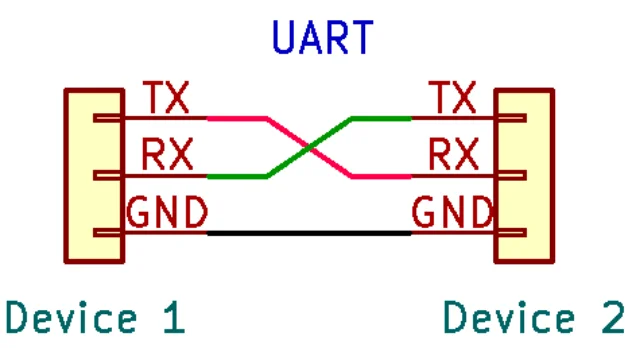
\includegraphics[width=0.8\textwidth]{Imagenes/Bitmap/uart}
        \caption{Ejemplo de conexión UART}
        \label{fig:uart}
    \end{figure}
    La línea TX de un dispositivo debe ir conectada a la línea RX del otro dispositivo, y la línea RX a TX.

    La comunicación es full dúplex, permitiendo la transmisión y recepción de datos de forma simultánea.
    Cada byte se transmite en una trama que incluye un bit de inicio (start bit), los bits de datos (normalmente 8), un bit opcional de paridad, y uno o más bits de parada (stop bits).

    Las velocidades de transmisión habituales van desde 9600 hasta 115200 baudios, aunque se pueden alcanzar velocidades de hasta 1 o 2 Mbps, dependiendo del hardware.

\end{itemize}

\begin{table}[h]
    \centering
    \footnotesize
    \renewcommand{\arraystretch}{1.1}
    \begin{tabular}{|l|c|c|c|}
        \hline
        \textbf{Característica}  & \textbf{SPI}               & \textbf{I²C}               & \textbf{UART}       \\
        \hline
        Tipo de comunicación     & Síncrona                   & Síncrona                   & Asíncrona           \\
        \hline
        Arquitectura             & Maestro-esclavo            & Maestro-esclavo            & Punto a punto       \\
        \hline
        Número de líneas         & 4 (CLK, CS, MOSI, MISO)    & 2 (SDA, SCL)               & 2 (TX, RX)          \\
        \hline
        Full/Half dúplex         & Full dúplex                & Half dúplex                & Full dúplex         \\
        \hline
        Número de dispositivos   & 1 maestro, varios esclavos & 1 maestro, varios esclavos & Solo dos            \\
        \hline
        Velocidad típica         & 1–10 Mbps                  & 100 kbit/s – 3.4 Mbit/s    & 9.6 kbit/s – 3 Mbps \\
        \hline
        Control de dirección     & Señal CS por esclavo       & Dirección en el protocolo  & No necesario        \\
        \hline
        Complejidad del hardware & Media                      & Baja                       & Muy baja            \\
        \hline
    \end{tabular}
    \caption{Comparativa entre las interfaces SPI, I²C y UART}
    \label{tab:comparativa_interfaces}
\end{table}


\section{Transmisión de datos mediante LoRa}


\section{Sensores embarcados: presión, orientación y GPS}


\section{Captura y transmisión de vídeo en tiempo real}


\section{Visualización de datos en tiempo real: arquitecturas orientadas a eventos}


\section{Modelado 3D de orientación con cuaterniones}